\chapter{Marco Teórico}
\raggedbottom

    \section{[n]-Triangulenos}
La definición para el conjunto de moléculas No-Kekulé de capa abierta y conjugación $\pi$ caracterizadas por ser unidades triangulares de hojas de grafeno, como es el fenalenil, simplemente trianguleno o sistemas de trianguleno $\pi$-extendidos \cite{morita2011synthetic, das2016polyradical}, se le conoce como [n]-trianguleno. Que como se puede hacer notar en la \Cref{fig:ntriangulenes}, siguen un patrón basado en la extensión de la longitud de lado del fragmento triangular.\\
\begin{figure}[htb!]
    \centering
    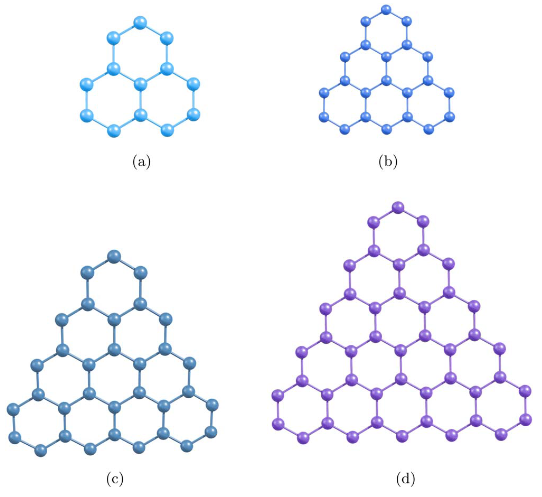
\includegraphics[width=0.5\linewidth]{triangulenes.png}
    \caption{Gráfica Molecular de [n]-triangulenos de dimensión, (a) n = 2, (b) n= 3, (c) n = 4, (d) n = 5 \cite{jyothish2024topological}.}
    \label{fig:ntriangulenes}
\end{figure}

        \subsection{Historia y primeras caracterizaciones}
El término trianguleno, previamente conocido como \textit{hidrocarburo de Clar}, se acuña originalmente del trabajo prístino de E. Clar y D. G. Stewart, donde menciona como la estructura No-Kekulé del trianguleno y que así como algunos de los derivados, denotaba una enorme inestabilidad e inmediata polimerización en otros compuestos \cite{clar1953aromatic}.\\
La breve historia del proceso de generación del trianguleno que parte desde 1953 es descrita apropiadamente por \textcite{valenta2022taming}, recopilando el trabajo de 70 años de múltiples investigadores desde que Clar hipotetizó esta estructura hasta la combinación de las técnicas in-solution y on-surface. El llamado de atención por el trianguleno es inmediato por los autores del principio, aunque Clar falla en sintetizarla no sin antes dejar un compuesto potencial para futuros trabajos, se menciona \textcite{HARA19772435} y el altamente simétrico dianión de trainguleno que practicamente era de los principales precursores in-solution del trianguleno descrito por Clar; no solo se mejoraron los resultados finales, el trabajo de \textcite{bushby1993esr} en 1993, hace una mejora en facilitar eficientemente uno de los compuestos precursores del trianguleno además mejora su almacenamiento y perdurabilidad.\\
Ya entrando en el siglo XXI, en 2019 hay reportes de las mejoras en la rapidez de la síntesis comparados con los procedimientos de Clar y Bushby et al. reduciendo el número de pasos en que se generaban los precursores del trianguleno así como su elaboración a gran escala \cite{ribar2019gram, holt2019short}. Cabe mencionar que la evolución descrita hasta ahora se hace enfocando solo el trabajo únicamente en reacciones químicas para para la obtención de todos estos compuestos y derivados; sin embargo, un par de años antes se implementaba una combinación histórica con técnicas on-surface y aislamiento de ultra alto vacío, es decir, manipulación atómica posibles con tecnología STM/ATM \cite{pavlivcek2017synthesis}, donde ya se tiene el propósito de esto es generar un precursor lo suficientemente cercano a la molécula de [3]-trianguleno con algunos métodos anteriormente utilizados para otros trabajos de \citeauthor{ribar2019gram} combinados con \citeauthor{holt2019short} para posteriormente aplicar voltajes y modificar la estructura de la molécula para obtener el resultado deseado del trianguleno.\\
Desde el reporte de este resultado, comenzó a ser posible obtener triangulenos para una dimensionalidad mucho mayor, desde el inicial [3]-trianguleno y hasta el más grande de sus homólogos [7]-trianguleno sintetizado en 2021, gracias a esta combinación de técnicas \cite{valenta2022taming}.\\
La importancia de estos avances la concluyen apropiadamente \textcite{pavlivcek2017synthesis} con el [3]-trianguleno y es que muestra ser un candidato prometedor para experimentos de resonancia en estados de espín del electrón para aplicaciones en espintrónica, ya que hay aspecto que se van conservando a medida que estudia los [n]-triangulenos aislados y es que esta familia No-Kekulé mantiene el incremento en su número de electrones desapareados (N) en función de n (Anillos laterales bencenoides), siguiendo la regla: $N = n - 1$, con un comportamiento único puesto que posee una densidad espinorial distribuida alrededor de toda la molécula y que se distingue de otro tipo de radicales típicos cuyo electrón desapareado está localizado en un solo átomo, ofreciendo oportunidades para el control de sus propiedades magnéticas a partir de modificaciones químicas \cite{jyothish2024topological}.\\
Se preve por la regla de Ovchinnikov para nanografenos que el estado fundamental de estas moléculas presentan la mayor multiplicidad de espín posible \cite{valenta2022taming}, entendiendo que esta regla establece que debido a efectos topológicos, el número cuántico de espín S del estado fundamental de una molécula aromática policíclica de hidrocarburo (PAH) es expresada como $S = |N_A-N_B|/2$ \cite{das2016polyradical}, donde A y B son los subsistemas $\pi$ del total de la red \Pref{fig:subsistemasPAH}.
\begin{figure}[thb!]
    \centering
    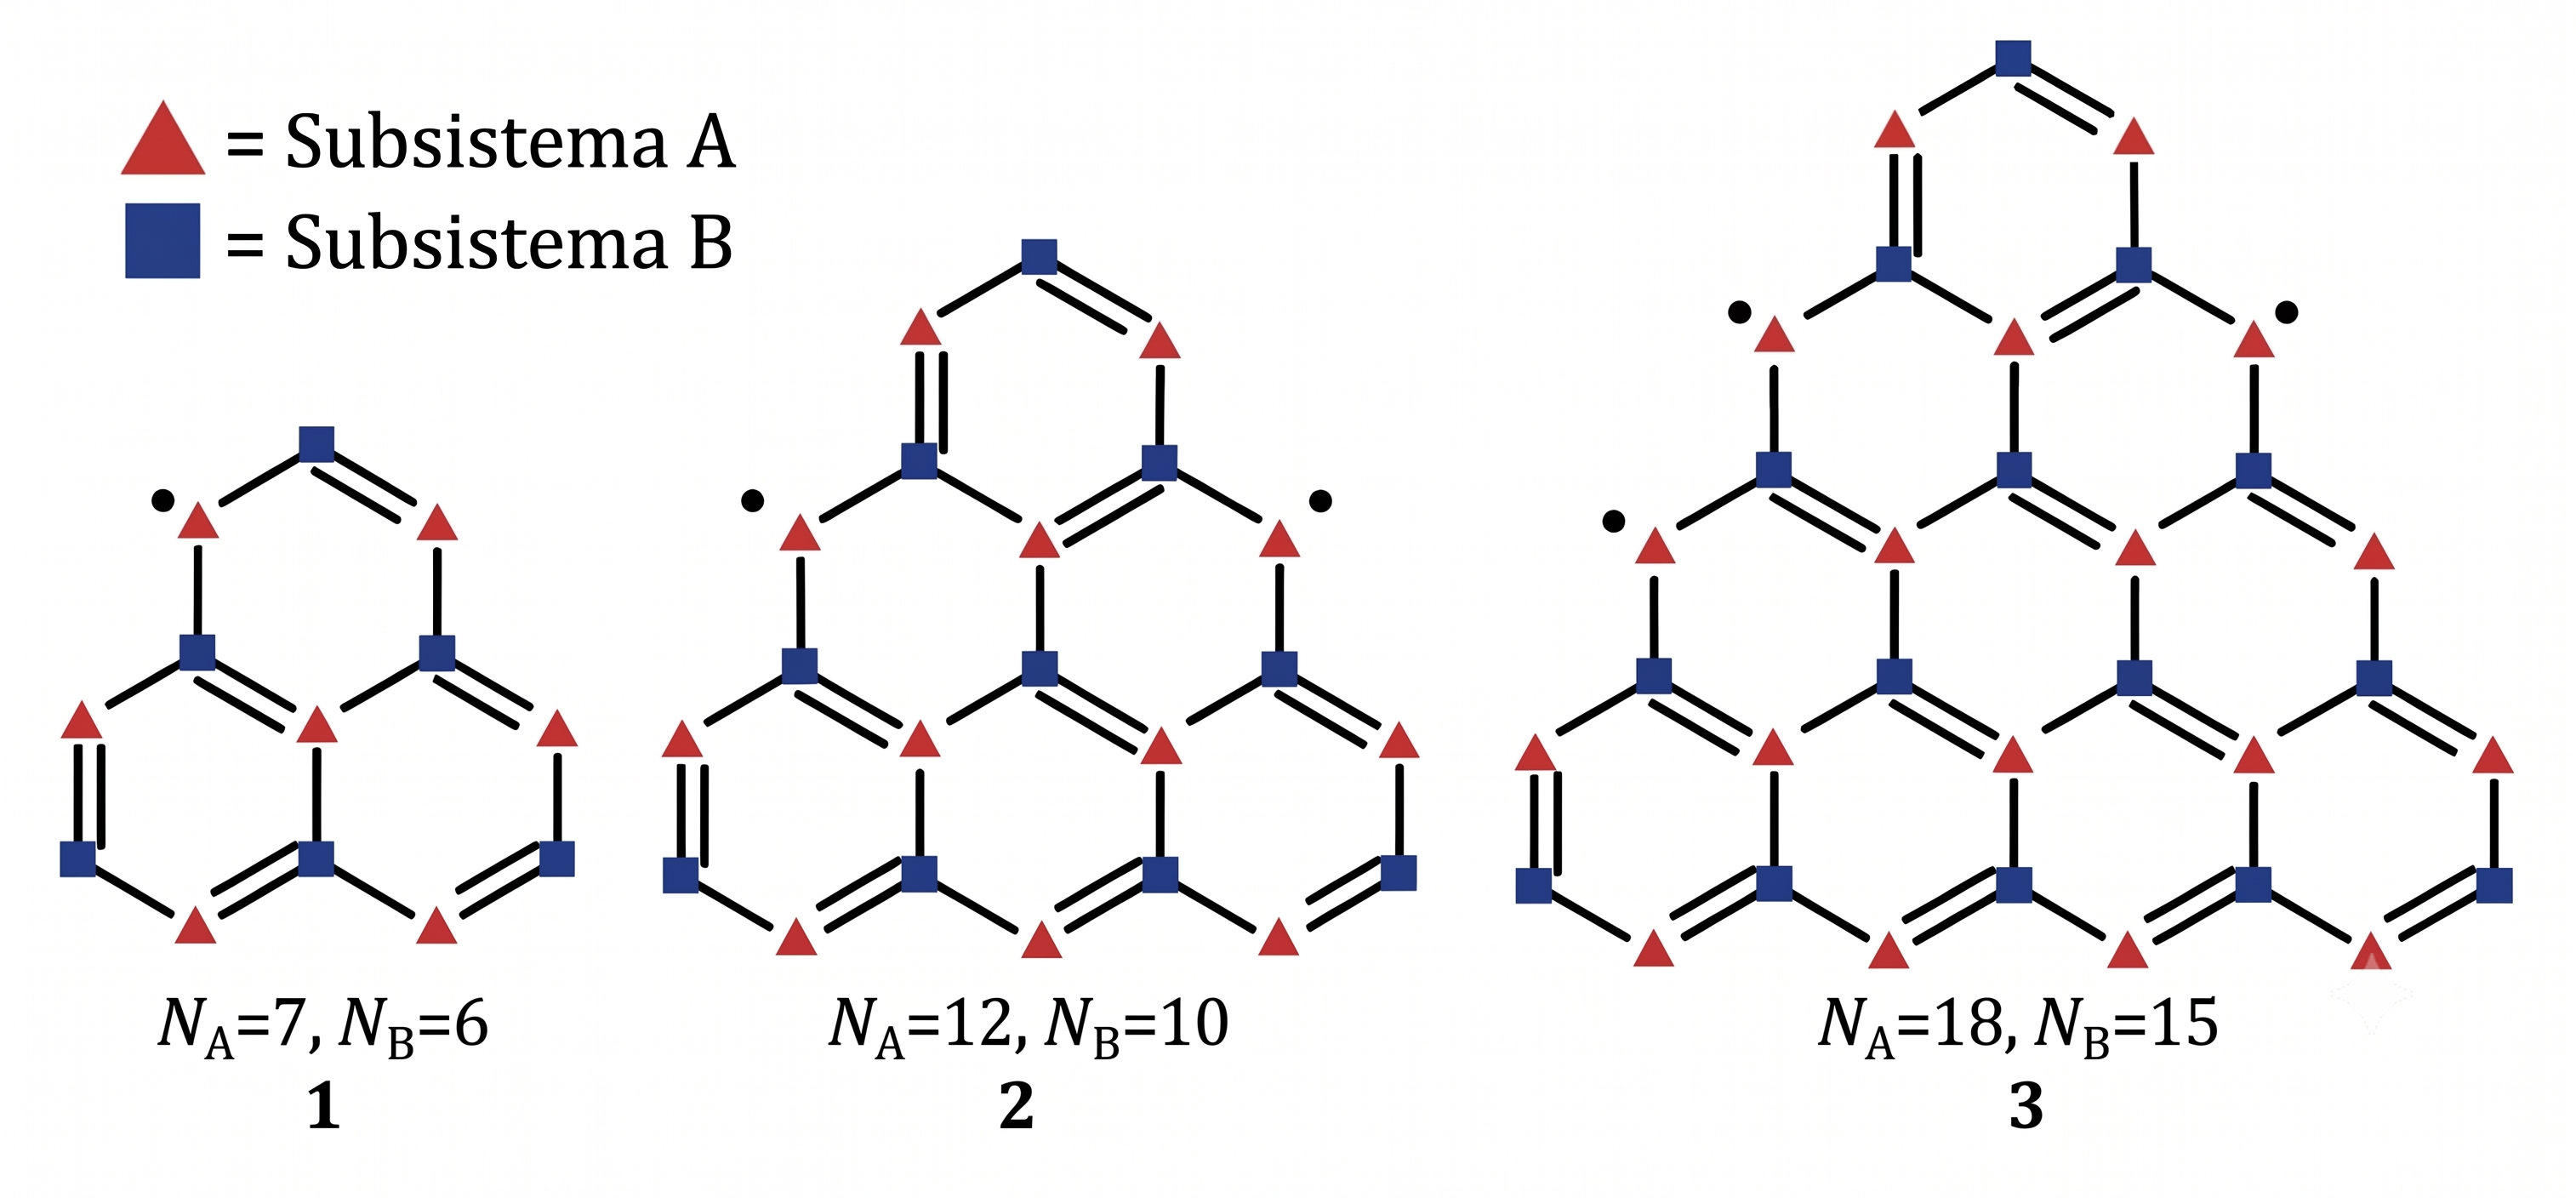
\includegraphics[width=0.8\linewidth]{Subsistemas.png}
    \caption{Estructura de triangulenos de dimensión n = 1, 2 y 3 con la distinción entre sus dos subsistemas $\pi$.}
    \label{fig:subsistemasPAH}
\end{figure}
        \subsection{Origen de las propiedades magnéticas}
        En electrónica molecular, surge el interés por moléculas de capa abierta inicialmente ya que denota un carácter magnético total no nulo bastante llamativo, sin embargo hay aspecto más fundamentales e inherentes a los [n]-triangulenos que deben el surgimiento de estos electrones $\pi$ con espin desapareado\cite{calupitan2023emergence}, se menciona:
        \begin{enumerate}
            \item La presencia de \textit{frustraciones topológicas} y el \textit{desequilibrio entre subredes} mantiene electrones de capas externas desapareados. En consecuencia, se ha encontrado una alta correlación entre descriptores moleculares asociados a teoría de grafos (usados para caracterizar la estructura de moléculas) con la energía de electrones $\pi$ y energía de deslocalización, elemento destacable por el creciente número de electrones desapareados. Este hecho, permite asociar un modelo predictivo muy preciso entre la estructura molecular y la energía de esta familia \cite{jyothish2024topological}. 

            \item Calculos realizados por \textcite{das2016polyradical} muestran que pese a que la densidad del estado base se distribuye en alguna de los redes (Subsistema \tikz[baseline=-0.2ex]\fill[red] (0,0) -- (0.24,0) -- (0.12,0.208) -- cycle; o \tikz[baseline=-0.2ex]\fill[blue] (0,0) -- (0.24,0) -- (0.24,0.24) -- (0,0.24) -- cycle;), tiene una mayor presencia en los bordes, propiedad compartida independientemente del tamaño. Ciertamente, la hipótesis que se mostraba partía de la idea de que PAHs de borde zigzag denotaban este comportamiento, pero resulta particularmente relevante ya que en una acumulación de electrones representa efectos de repulsión de Coulumb y en combinación con exclusión de Pauli, tienen como consecuencia que en los estados de baja energía (respecto al nivel de Fermi) haya \textit{polarización de espín}, es decir, un número $n$ de electrones $\pi$ cuyo espin se encuentra alineado en la misma dirección.
        \end{enumerate}
        En definitiva, el magnetismo de los [n]-triangulenos tiene origenes no triviales que ha sido bien reportado en la literatura a nivel teórico y experimental, algunos incluyen cambios en los componentes de la molécula, usarla como bloque de construcción para sistemas más grandes, acoplarla a superficies metálicas, entre otras \cite{das2016polyradical, calupitan2023emergence,turco2024magnetic, wang2022aza}.
        \subsection{Potencial para transporte electrónico}
        Con respecto a comprender el fenómeno de transporte electrónico a nivel molecular, se aclara en principio que comprende un área bastante amplia, que se plantea equiparar el comportamiento de los múltiples componentes electrónicos que son usados a día de hoy, pero trabajando con moléculas individuales o grupos de ellas. En este sentido, se tiene multiples opciones para trabajar en la generación de la arquitectura de un dispositivo molecular, sin Sin embargo desde un principio el candidato más prominente por sus propiedades particulares, es el carbono y moléculas compuestas por este elemento en su mayoría que no son pocas, desde hidrocarburos, cristales o estructuras de grafeno, como son nanotubos, fullerenos, entre otros.\\
        \textcite{cuevas2017molecular} hacen una revisión de aspectos primarios que debería satisfacer un sistema de transporte electrónico en términos de funcionalidades de algunos componentes básicos, puntualizando la labor de moleculas como alcanos, alquenos, alquinos, aromáticos e incluye una mencion de los PAHs, que son de particular interés en este trabajo.\\
        
    \section{Sistema de Transporte}
        \subsection{Conexiones}
        \subsection{Grupos funcionales}
    \section{Espintrónica}
    \section{Filtrado de electrones}